
%%%%    IMPORTS 2 BASE    %%%%


\documentclass[hidelinks, french, oneside]{article}
\usepackage[utf8]{inputenc}
\usepackage[T1]{fontenc}

% pour le mise en page
\usepackage[a4paper, total={6.5in, 10in}]{geometry}
\usepackage{fontsize} \changefontsize[13]{10}		
\usepackage{xcolor}

% mathsymbole
\usepackage{amsmath, amssymb,stmaryrd}
\usepackage{wasysym}[mathcal] % a quoi sert le [mathcal] ?
\usepackage{nicefrac, units} % fraction pour text mode / unité

% TBD
\usepackage{mathcomp}
\usepackage{mathrsfs} % pour \mathscr a priori

% pour les belles fonts
\usepackage{amsfonts}
\DeclareMathAlphabet{\mathpzc}{OT1}{pzc}{m}{it}
%\usepackage{euscript}[mathcal]
%\usepackage{rsfso}
\usepackage{bbm}	 % mathbb étendu

% pour les hyprlien / cross-ref
\usepackage{hyperref, cleveref}
%\namecref{sec:label}

%pour les figures
\usepackage{graphicx} \usepackage{wrapfig, floatrow}
%\usepackage{subcaption} % surement useless, parsk floatrow-like 

% pour les beaux tableaux
\usepackage{multirow}

% pour des matrices infernales
\usepackage{easybmat}

% pour les citations (aucune idées de comment ca marche)
\usepackage{csquotes}



%%%%    RACCOURCIS    %%%%


% bb / cal / frak
\newcommand{\N}{\mathbb{N}}
\newcommand{\Z}{\mathbb{Z}}             % Note pour homo pour les updates
\newcommand{\Q}{\mathbb{Q}}
\newcommand{\R}{\mathbb{R}}
\newcommand{\C}{\mathbb{C}}
\newcommand{\K}{\mathbb{K}}
\renewcommand{\k}{\Bbbk}
\newcommand{\U}{\mathbb{U}}
\renewcommand{\u}{\text{U}}
\newcommand{\A}{\mathbb{A}}
\newcommand{\T}{\mathscr{T}}
\newcommand{\I}{\mathbb{I}}
\newcommand{\one}{\mathbbm{1}}
%\renewcommand{\S}{\mathfrak{S}}
\renewcommand{\S}{\mathbb{S}}

% arrows
\newcommand{\lr}{\longrightarrow}
\newcommand{\Lr}{\Longrightarrow}
%\renewcommand{\ll}{\longleftarrow}
\newcommand{\Ll}{\Longleftarrow}
\newcommand{\llr}{\longleftrightarrowr}
\newcommand{\Llr}{\Longleftrightarrow}

% espaces
\newcommand{\matk}{\mathpzc{M}_n(\mathbb{K})}
\newcommand{\matr}{\mathpzc{M}_n(\mathbb{R})}

% fonctions
\newcommand{\Arccos}{\text{Arccos}} 
\newcommand{\Arcsin}{\text{Arcsin}} 
\newcommand{\Arctan}{\text{Arctan}} 
\newcommand{\Argch}{\text{Argch}}       
\newcommand{\Argsh}{\text{Argsh}}

\newcommand{\congu}[1]{\overline{#1}}
\newcommand{\argmin}[1]{\underset{#1}{\text{argmin}}}
\newcommand{\argmax}[1]{\underset{#1}{\text{argmax}}}

\newcommand{\pgcd}{\text{pgcd}}
\newcommand{\PGCD}{\text{PGCD}}
\newcommand{\ppmc}{\text{ppcm}}
\newcommand{\sign}{\text{sign}}

\newcommand{\sgn}{\text{sgn}}
%\newcommand{\deg}{\text{deg}}
\newcommand{\ord}{\text{ord}}
\newcommand{\rot}{\text{rot}}

%\renewcommand{\det}{\text{det}}
\newcommand{\tr}{\text{tr}}
\newcommand{\rg}{\text{rg}}
\newcommand{\Co}{\text{com}}
\newcommand{\codim}{\text{codim}}

%espaces
%\renewcommand{\Vec}{\text{Vec}}
\newcommand{\im}{\text{Im}}
\newcommand{\Ker}{\text{Ker}}
\newcommand{\Ann}{\text{Ann}}
\newcommand{\Sp}{\text{Sp}} 
\newcommand{\GL}{\text{GL}}
\newcommand{\SL}{\text{SL}}
\newcommand{\SO}{\text{SO}}
\newcommand{\SU}{\text{SU}}
%\renewcommand{\div}{\text{div}}

\newcommand{\Aff}{\text{Aff}}
\newcommand{\HT}{\text{HT}}
\newcommand{\GA}{\text{GA}}

% spé proba
\newcommand{\esp}[2][]{\mathbb{E}_{#1}\left[\, #2\, \right]}
\newcommand{\var}[2][]{\mathbb{V}_{#1}\left[\, #2\, \right]}
%\newcommand{\Var}{\mathbb{V}}%\text{ar}}

% plus jolie
\renewcommand{\O}{\varnothing}
\renewcommand{\epsilon}{\varepsilon}
\renewcommand{\subsetneq}{\varsubsetneq}
\renewcommand{\leq}{\leqslant}
\renewcommand{\geq}{\geqslant}
\renewcommand{\limsup}{\varlimsup}
\renewcommand{\liminf}{\varliminf}

% autre
\newcommand{\defeq}{:=}
\renewcommand{\bf}[1]{\boldsymbol{#1}}
\renewcommand{\AC}{\sim}
\newcommand{\para}{\sslash}


% latin
\newcommand{\etal}{\textit{et al.}}
\newcommand{\etc}{\textit{etc.}}
\newcommand{\apriori}{\textit{a priori}}
\newcommand{\afortiori}{\textit{a fortiori}}
\newcommand{\acontrario}{\textit{a contrario}}
\newcommand{\infine}{\textit{in fine}}
\newcommand{\ie}{\textit{i.e.}}
\newcommand{\eg}{\textit{e.g.}}

% tmp
\newcommand{\phaset}{\Phi_{\text{tot}}}
\newcommand{\phased}{\Phi_{\text{dyn}}}
\newcommand{\phaseg}{\Phi_{\text{geo}}}



%%%%    ENONCES (PROP, DEF, RQ)    %%%%


\usepackage{amsthm}

% les styles
\newtheoremstyle{enonce}{0pt}{25pt}{}{}{\scshape}{\quad ---\quad }{0em}{}
\newtheoremstyle{special}{0pt}{25pt}{}{}{\scshape}{\quad ---\quad }{0em}{\thmnote{#3}}
\newtheoremstyle{rqlike}{0pt}{25pt}{\itshape}{}{\scshape}{\quad ---\quad}{0em}{}
\newtheoremstyle{exo}{0pt}{25pt}{\color{blue}}{}{\scshape\color{blue}}{: \newline}{0em}{}

% énoncés classiques
\theoremstyle{enonce}
\newtheorem{definition}{Définition}
\newtheorem{proposition}{Proposition}
\newtheorem{propriete}{Propriété}
\newtheorem{propricarac}[propriete]{Propriété Caractéristique}
\newtheorem{lemme}{Lemme}
\newtheorem{theoreme}{Théorème}[section]
\newtheorem{theodef}[theoreme]{Théorème et Définition}
\newtheorem{corollaire}{\qquad Corollaire}[theoreme]

% énoncé type
\theoremstyle{special}
\newtheorem{enonce}{}

% énoncé numérotation-less
\theoremstyle{rqlike}
\newtheorem*{remarque}{\qquad Remarque}
\newtheorem*{rappel}{\qquad Rappel}
\newtheorem*{exemple}{\qquad Exemple}

\theoremstyle{exo}
\newtheorem{exercice}{Exercice}

% pour cref aux enoncés
\crefname{definition}{définition}{Définition}
\crefname{proposition}{proposition}{Proposition}
\crefname{propriete}{propriété}{Propriété}
\crefname{lemme}{lemme}{Lemme}
\crefname{theoreme}{théorème}{Théorème}
\crefname{corollaire}{corollaire}{Corollaire} 

\crefname{remarque}{remarque}{Remarque}
\crefname{rappel}{rappel}{Rappel}
\crefname{exemple}{exemple}{Exemple}

\crefname{exercice}{exercice}{Exercice}

% espace démo  (pas convaincu)
\definecolor{mygray}{gray}{0.3}
\newtheoremstyle{demo}{8pt}{0pt}{\color{mygray}}{}{\itshape\color{mygray}}{\newline\newline}{0em}{}

\theoremstyle{demo}
\newtheorem*{demo}{\qquad\qquad\qquad\rule{3.5cm}{0.4pt}\qquad\quad Démonstration\qquad\quad \rule{3.5cm}{0.4pt}}
%\begin{center}\rule{8cm}{0.4pt}\end{center}



%%%%    PROG N PLOT    %%%%


% Prog

%\usepackage{fancyvrb} % pour le lore, mais useless AF
\usepackage{listings} 
\usepackage{pythontex}	% surement une dingz, à approfondire

% preset
\definecolor{codeblack}{gray}{0.2}
\definecolor{codegreen}{rgb}{0,0.6,0}
\definecolor{codegray}{gray}{0.5}
\definecolor{codepurple}{rgb}{0.58,0,0.82}
\definecolor{backcolour}{rgb}{0.98,0.98,0.95}

\lstdefinestyle{mystyle}{
backgroundcolor=\color{backcolour},   
commentstyle=\color{codegray},
keywordstyle=\color{orange},
numberstyle=\tiny\color{codegray},
stringstyle=\color{codegreen},
basicstyle=\color{codeblack}\ttfamily\footnotesize,
breakatwhitespace=false,         
breaklines=true,                 
captionpos=b,
abovecaptionskip=12,
belowcaptionskip=18,
keepspaces=true,                 
numbers=left,                    
numbersep=5pt,                  
showspaces=false,                
showstringspaces=false,
showtabs=false,                  
tabsize=2,
frame=single,
rulecolor=\color{lightgray}}
\lstset{style=mystyle}


% Plot

% pour dessins et les diagrams
\usepackage{tikz, tikz-cd, tkz-euclide}
\usepackage{scalerel, pict2e}
\usetikzlibrary{calc, patterns, shapes.arrows, arrows.meta, shadows, external} 

% pour les maxis plots
\usepackage{pgfplots}
\pgfplotsset{compat=newest, scaled y ticks=false}
\usepgfplotslibrary{groupplots, dateplot, statistics, fillbetween}

\tikzstyle{every node}=[font=\scriptsize]
\pgfplotsset{standard/.style={width=8cm,
	height=3cm,
	compat=1.18,
	trig format=rad,
	enlargelimits,
	axis x line=middle,
	axis y line=middle,
	enlarge x limits=0.15,
	enlarge y limits=0.15,
	every axis x label/.style={footnotesize, at={(current axis.right of origin)},anchor=north west},
	every axis y label/.style={footnotesize, at={(current axis.above origin)},anchor=south east},
	scale only axis=true}}
	
	
	
	%%%%    CAPTIONS 2 FIGURES    %%%%
	
	
	% set up des captions figures (extrêmement BG)
	
	% pos et séparateur générale
	\captionsetup{justification=centering}
	\DeclareCaptionLabelSeparator{custom}{\, ---\, }
	
	% spécial figure
	\DeclareCaptionLabelFormat{customfig}{\textit{fig. #2}}
	\DeclareCaptionFormat{customfig}{#1#2#3}
	%\DeclareCaptionFont{customfig}{\itshape} %marche pas jsppk
	\renewcommand{\thefigure}{\arabic{section}.\arabic{figure}}
	\captionsetup[figure]{labelformat=customfig, labelsep=custom}
	
	% spécial code (listings)
	\DeclareCaptionLabelFormat{customcode}{\textit{code \arabic{section}.#2}}
	\DeclareCaptionFormat{customcode}{#1#2#3}
	%\renewcommand{\thelstlisting}{\arabic{section}.\arabic{lstlisting}}
	\captionsetup[lstlisting]{labelformat=customcode, labelsep=custom}
	
	
	
	%%%%    TABLES/REF  &  HAUT/BAS DE PAGES    %%%%
	
	
	% nom des tables et références
	
	\renewcommand{\contentsname}{\begin{center}\textsc{Tables des Matrières}\end{center}}
	\renewcommand{\listfigurename}{\begin{center}\textsc{Table des Figures}\end{center}}
	\renewcommand{\lstlistlistingname}{\begin{center}\textsc{Table des Codes}\end{center}}
	\renewcommand{\refname}{\begin{center}\textsc{Références}\end{center}}
	
	% bas/haut de page (à optimiser à l'occas')
	
	\usepackage{fancyhdr}
	\pagestyle{fancy}                       
	\fancyhf{}
	\renewcommand{\headrulewidth}{0pt}
	\cfoot{\thepage}
	
	%version2réjane  :
	%\usepackage{eso-pic}
	%\renewcommand\headrulewidth{1pt}
	%\fancyhead[L]{\includegraphics[width=3cm]{logo_lr.png}}
	%\fancyhead[R]{\includegraphics[width=1cm]{logo_sdis17.png}}
	%\setlength{\headsep}{45pt}
	
	
	
	%%%%    SECTIONS ET TOC    %%%%
	
	
	% génération des sections
	
\usepackage[loadonly, toctitles, clearempty, newparttoc]{titlesec}

% liste des sections
\titleclass{\part}[0]{top} % 0 = niveau de section
\titleclass{\section}{straight}[\part]
\titleclass{\subsection}{straight}[\section]
\titleclass{\subsubsection}{straight}[\subsection]

% génère les numérotations avec format
%\newcounter{part}
\renewcommand{\thepart}{\Roman{part}}
%\newcounter{section}
\renewcommand{\thesection}{\Roman{section}}
%\newcounter{subsection}
\renewcommand{\thesubsection}{\arabic{section}.\arabic{subsection}}
%\newcounter{subsubsection}
\renewcommand{\thesubsubsection}{\arabic{section}.\arabic{subsection}.\arabic{subsubsection}}

% formatage
\titleformat{\part}[display]{\bfseries\scshape\Large}{\centering \rule{3.5cm}{0.4pt}\qquad Chapitre\quad \thepart \qquad \rule{3.5cm}{0.4pt}}{15pt}{\centering}[\vspace{0.2cm}\rule{8cm}{0.4pt}]
\titlespacing{\part}{0pt}{50pt}{70pt}
\newcommand{\partbreak}{\clearpage}

\titleformat{\section}{\bfseries\Large}{\thesection\quad ---}{15pt}{}
\titlespacing{\section}{10pt}{20pt}{15pt}
%\newcommand{\sectionbreak}{\clearpage}

\titleformat{\subsection}{\bfseries\large}{\thesubsection}{15pt}{}
\titlespacing{\subsection}{20pt}{15pt}{15pt}

\titleformat{\subsubsection}{\bfseries}{\thesubsubsection}{15pt}{}
\titlespacing{\subsubsection}{30pt}{15pt}{15pt}

% pour cref aux enoncés
\crefname{part}{partie}{Partie}
\crefname{section}{section}{Section}
\crefname{subsection}{sous-section}{Sous-section}


	% le TOC en lé-gende

\usepackage{titletoc}
%\contentsmargin{2em}

\titlecontents{part}[2em]{\bfseries\large\scshape 
	\hspace*{-1.5em}\rule{\textwidth}{0.5pt}\vspace{0.1cm}\\*
	 }{Chaptire\quad \contentslabel{-0.05em}\quad\ ---\quad}{\contentslabel{-1.5em} ---\quad }{\hfill\contentspage}[\hspace*{-0.5em}
\rule{\textwidth}{0.5pt}]

\titlecontents{section}[1.5em]{\addvspace{1em}\bfseries}{\contentslabel{1.25em} ---\quad}{\hspace*{-1.75em}}{\titlerule*[0.75pc]{.}\contentspage}[\addvspace{0.25em}]

\titlecontents{subsection}[3.8em]{\addvspace{0.15em}\normalfont}{\contentslabel{2em}}{\hspace*{-2em}}{\titlerule*[0.75pc]{.}\contentspage}

\titlecontents{subsubsection}[6.8em]{\normalfont}{\contentslabel{2.75em}}{\hspace*{-2.5em}}{\titlerule*[0.75pc]{.}\contentspage}


% set up d'un environnement pour les annexes

\newenvironment{annexe}{%
	\newpage
	
	% changement title sec
	\titleformat{\section}[display]{\bfseries\scshape\Large}{\centering}{15pt}{\centering}
	\titlespacing{\section}{0pt}{30pt}{40pt}
	
	\titleformat{\subsection}{\bfseries\large}{Annexe \thesubsection\quad ---\quad}{0pt}{}
	
	\titleformat{\subsubsection}{\bfseries}{\thesubsubsection}{15pt}{}
	
	% changement title toc
	\titlecontents{section}[0.25em]{\addvspace{0.5em}\bfseries}{}{\hspace*{-1.5em}}{\titlerule*[0.75pc]{.}\contentspage}
	
	\titlecontents{subsection}[1.5em]{\normalfont Annexe\hspace*{2.5em}}{\contentslabel{2em}}{\hspace*{-2em}}{\titlerule*[0.75pc]{.}\contentspage}
	
	\titlecontents{subsubsection}[6em]{\normalfont}{\contentslabel{2.75em}}{\hspace*{-2em}}{\titlerule*[0.75pc]{.}\contentspage}
	
	% changment de la numéritations
	\renewcommand{\thesubsection}{\Alph{subsection}}
	\renewcommand{\thesubsubsection}{\Alph{subsection}.\arabic{subsubsection}.}
	% mise à zéro des compters
	%\setcounter{section}{0}
}{}


\begin{document}


\begin{titlepage}
	%\AddToShipoutPictureBG*{\put(80,655){\includegraphics[width=2.9cm]{Logo MIX.png}}}
	%\AddToShipoutPictureBG*{\put(70,738){\includegraphics[width=5cm]{logo_lr.png}}}
	%\hspace{0.0cm} 
	%\AddToShipoutPictureBG*{\put(440,690){\includegraphics[width=3.0cm]{logo_sdis17.png}}}\\[5.0cm]
	%{\color{white}l}\par
	
	\centering
	\vspace{1.5cm}
	{\huge\textbf{Rapport de Stage de M2}}\par
	
	\vspace{2cm}
	{\huge\textbf{\textsc{Des trucs sûrement très cools}}}\par 
	\vspace{0.5cm}
	
	{\huge\textbf{\textsc{vraiment très très cool}}}\par
	\vspace{2.0cm}
	
	{\large Grégoire \textsc{Doat}}\par
	\vspace{0.5cm}
	\vfill
	
	% Bottom of the page
	{\large Encadré par Nicolas \textsc{Le Bihan},  Michel \textsc{Berthier}, \etal}\par
	\vspace{0.5cm}
	
	\rule{10cm}{0.4pt}\par
	\vspace{0.7cm}
	
	{Master \textsc{Mix} - Université de La Rochelle}\par
	\vspace{0.25cm}
	
	{\large 2024 - 2025}
\end{titlepage}

\newpage
\tableofcontents
\thispagestyle{empty}
{\color{white}l}


\newpage
\setcounter{page}{1}



\newpage

\phantomsection
\addcontentsline{toc}{section}{Introduction}
\section*{Introduction}

Quote : The geometric phase is also one of the most beautiful examples of what Wigner once called ``the unreasonable effectiveness of mathematics in the natural sciences.'' \cite[p.\,4]{bohm_geometric_2003}

Des questions :
\begin{itemize}
	
	\item Pourquoi on va dans les complexes ? Réponse \cref{sec:temp-freq}
	
	\item Pourquoi Schrödinger ? Peut-être que Mukunda \cite{mukunda_quantum_1993} à la réponse
	
	\item En quoi la phase géométrique est une phase ? lien avec Fourier ?
	
	\item Lien entre phase et polarisation : différences, intérêts ? C'est une phase dans la polar IMO
	
	\item La param $(a,\chi,\theta,\varphi)$ elle dit quoi vraiment ? (sûrement simple à généraliser btw) + $(\chi,\theta)$ est pas en bijection avec la sphère (surement osef par contre)
	
	\item Multivaluation dans les variétés \cite[p. 8]{bohm_geometric_2003} ???
	
\end{itemize}

\[\underline{\overline{\qquad\qquad\qquad\qquad\qquad\qquad\qquad\qquad\qquad\qquad\qquad\qquad\qquad\qquad\qquad\qquad\qquad\qquad}}\]{\color{white}relbinrei}

Note de rédac :
\begin{itemize}
	\item Index ? rappel $\delta$ de Dirac
\end{itemize}


\part{Transformation en Signal Analytique}




\begin{enonce}[Intro de la \cref{sec:temp-freq}]
	\textit{Malgré ce que l'énoncé de la problématique laisse entendre, dans toute la suite nous travaillerons avec des signaux à valeur de $\R$ dans $\C^n$ plutôt que $\R^n$. Il y a de très bonne raison à la transformation des signaux réels en complexes et c'est sera l'objet de cette première  \namecref{sec:temp-freq}.}\\
	
	Et pourquoi on veut faire du temps fréquence aussi ? (t'explique pourquoi c'est bien mais pourquoi ca NOUS intéresse ?)
\end{enonce}



%\section{Signal analytique, transformé de Hilberts, Analyse en temps-fréquence}
\section{Sur l'intérêt de transformé les signaux réels en complexes}\label{sec:temp-freq}


\textit{Cette partie reprends, dans les grandes lignes, les propos de \textsc{Cohen} dans son livre \emph{Time frequency analysis} \cite{cohen_time_1995}}
\\
Dans l'étude de signaux, la transformée de Fourier est un outil standard puisqu'il donne accès à tout l'information fréquentielle de ce dernier. Ce gain d'information n'est pas gratuit pour autant puisqu'on perd avec tout notion de temporalité. Pourtant dans bien des cas, une information instantanée, dépendante en temps, est plus pertinente.
\\
C'est par exemple le cas dans l'étude de la langue oral (bon terme ?). Le sens d'une phrase ne vient pas du signal, \ie~la voix, tout entier mais plutôt de ses valeurs locales. Lorsque l'on prononce le mot ``\textit{fleur}'', c'est l’enchaînement des sons associés au ``\textit{f}'', ``\textit{l}'', ``\textit{eu}'', \etc~qui est important et non la structure global du signal.  
\\
On pourrait également cité l'effet Döppler qui permet, entre autre, de savoir si un émetteur s'éloigne ou se rapproche. Dans ce cadre, le passage d'un signal de hautes à basses fréquences (typiquement d'un son aigu à un son grave) indique que la source, qui se rapprochait, s'est mise à s'éloigner : c'est la variation de fréquence en cours du temps qui est porteuse d'information.
\\

Pour avoir une notion de fréquence instantanée, il serait utile de pouvoir écrire tout signal réel $x$ sous la forme :
\begin{equation}\label{eq:amp-phase_instant}
	x(t) = a(t) \cos\phi(t)
\end{equation}
\\
où $a$ correspondrait à l'\textit{amplitude instantanée} du signal et $\phi$ sa \textit{phase instantanée}. Le problème d'une telle décomposition est que, si elle existe bel et bien, elle n'est en revanche pas unique. L'exemple le plus simple étant le cas $\ x(t) = \sin(t)\ $ qui se représente, entre autre, par les pairs :
\begin{align*}
	\big(a(t),\phi(t)\big) &= \big(1, t+\nicefrac{\pi}{2}\big)  &  
	\big(a(t),\phi(t)\big) &= \big(\sin(t), 0\big)  &  
	\big(a(t),\phi(t)\big) &= \big(2\sin(\nicefrac{t}{2}), \nicefrac{t}{2}\big)
\end{align*}
{\color{white}l}

Pour avoir unicité de cette décomposition, il nous faut donc une contrainte sur $(a,\phi)$. Une approche serait de voir $x$ comme la partie réelle du signal complexe :
\[\forall t\in\R,\quad z_x(t) = a(t)e^{i\phi(t)}\ \ \Lr\ \ x(t) = \Re e\, z_x(t)\]
\\
Dans ce cas on aurait bien unicité de $a$ et $\phi$ par rapport à $z_x$ (son amplitude et sa phase) mais cela ne fait que déplacer le problème puisque $z_x$ n'est pas mieux défini : Il y a une liberté totale quant au choix sa partie imaginaire. Pour motiver la définition de $z_x$, sont rappeler quelques outils d'analyse temps-fréquence.



\subsection{Distribution de l'énergie en temps et fréquence}\label{subsec:distrib_temp-freq}

Dans toute cette \namecref{sec:temp-freq}, on considèrera $x$ un signal complexe et on notera $\hat{x}$ ou $\mathcal{F}(x)$ sa transformée de Fourier (dont on supposera quelle existe, ici on supposera au moins $x\in L^2(\R, \C)$) :
\begin{align*}
	x\ &:\quad \begin{aligned}\R\ &\lr\quad \C \\ x\ &\longmapsto\ x(t)
	\end{aligned}  &  \mathcal{F}(x)=\hat{x}\ &:\quad \begin{aligned}\R\ &\lr\qquad\quad \C \\ \nu\ &\longmapsto\ \int_\R x(t)e^{-2\pi i \nu t}dt
	\end{aligned}
\end{align*}
\\

\begin{definition}[Densités d'énergie]\label{def:densi_dE}
	Étant donnée un signal complexe $x$, la \emph{densité d'énergie} $\rho$ de $x$ est donnée par le carré de son module. De même on définit $\varrho$ la \emph{densité d'énergie spectrale} :
	\begin{equation}\label{eq:densi_dE}
		\begin{aligned}
			\rho\ &:\quad \begin{aligned}\R\ &\lr\quad \R^+ \\ t\ &\longmapsto\ \big|x(t)\big|^2 \end{aligned}  &
			\varrho\ &:\quad \begin{aligned}\R\ &\lr\quad \R^+ \\ \nu\ &\longmapsto\ \big|\hat{x}(t)\big|^2 \end{aligned}
		\end{aligned}
	\end{equation}
	\\
	La valeur $\rho(t)$ correspond à la puissance déployée pour émettre le signal à l'instant $t$ et $\varrho(\nu)$ à l'énergie associée à la fréquence $\nu$ sur tout le signal. 
	\\
	La transformée étant une isométrie de l'espace $L^2(\R,\C)$, si $x\in L^2(\R,\C)$, alors l'\emph{énergie totale} du signal est indépendante de la représentation de ce dernier (temporelle ou spectrale) :
	\begin{equation}\label{eq:parceval}
		E(x) \defeq {\|x\|_2}^2 = \int_\R \rho(t) dt = \int_\R \varrho(\nu) d\nu = {\|\hat{x}\|_2}^2
	\end{equation}
\end{definition}

Par exemple, si $\ x(t)=e^{2\pi i\nu_0 t}$, alors $\ \hat{x}(t) = \delta(x-\nu_0)$. Dans ce cas, on a les densités :
\begin{align*}
	\rho(t) &= 1  &  \varrho(\nu) = \delta(\nu-\nu_0)
\end{align*}
Du point de vu temporel, le signal est émis avec une puissance régulière, mais le fait que $\varrho$ soit un dirac indique que toute l'énergie du signal est concentré en une unique fréquence $\nu_0$.
\\ \\

\begin{definition}[Durée et largeur de bande]\label{def:band-width}
	L'espérance ces densités sont notées, pour peu qu'elles existent :
	\begin{align*}
		\esp[\rho]{t} &\defeq \int_\R t \big|x(t)\big|^2 dt   &  \esp[\varrho]{\nu} &\defeq \int_\R \nu \big|\hat{x}(\nu)\big|^2 d\nu
	\end{align*}
	\\
	Si un signal est localisé temporellement, alors la première espérance/moyenne donne une idée de l'instant d'émission du signal. Si \acontrario, le signal est localisé en fréquence, la seconde espérance peut s'interpréter comme la fréquence ''dominante'' du le signal, ou plus généralement comme sa \emph{fréquence moyenne}. \\
	En particulier, et ce sera important pour la suite, dans le cas des signaux réels, l'espérance de $\varrho$ est toujours nulles.
	\\
	On note de même les variances (toujours à condition d'existence) :
	\begin{align*}
		\var[\rho]{t} &\defeq \esp[\rho]{\big(t-\esp[\rho]{t}\big)^2}  &  \var[\varrho]{\nu} &\defeq \esp[\varrho]{\big(\nu - \esp[\varrho]{\nu}\big)^2}\\
		& = \esp[\rho]{t^2} - \esp[\rho]{t}^2  &  &= \esp[\varrho]{\nu^2} - \esp[\varrho]{\nu}^2
	\end{align*}
	Les écart-types associés sont plus facilement interprétable. Le premier est appelé \emph{durée d'émission} du signal, puisqu'il renseigne l'étalement temporelle du signal ; et le second \emph{largeur de bande (fréquentielle)} puisque, lui, renseigne l'étalement fréquentielle. 
\end{definition}



\subsection{Fréquence instantanée et covariance}

Pour ce qui va suivre, les formules \eqref{eq:moment_f} et \eqref{eq:moment_t} suivantes seront nécessaire :
\\

\begin{proposition}[``Calculation tricks'' de \cite{cohen_time_1995}] \label{prop:integ_trick}
	Si le signal est $n$ fois dérivable et que la densité d’énergie associée $\varrho$ admet un moment d'ordre $n$, alors il est donnée par la formule :
	\begin{equation}\label{eq:moment_f}
		\forall n\in\N,\qquad \esp[\varrho]{\nu^n} = \left(\frac{i}{2 \pi}\right)^n  \int_\R x(t) \frac{d^n}{dt^n} \congu{x(t)} dt = \left(\frac{i}{2 \pi}\right)^n  \left\langle x, \frac{d^n}{dt^n}x\right\rangle
	\end{equation}
	\\
	Avec les hypothèses analogues, les moments de $\rho$ s'écrivent :
	\begin{equation}\label{eq:moment_t}
		\forall n\in\N,\qquad \esp[\rho]{t^n} = \left(\frac{1}{2i \pi}\right)^n  \int_\R \hat{x}(\nu) \frac{d^n}{dt^n} \congu{\hat{x}(\nu)} dt = \left(\frac{1}{2i \pi}\right)^n  \left\langle \hat{x}, \frac{d^n}{d\nu^n}\hat{x}\right\rangle
	\end{equation}
	
	\begin{demo}
		\`A supposer que les intégrales existes et que le théorème de Fubini s'applique, on a $\forall n\in\N$ :
		\begin{align*}
			\esp[\varrho]{\nu^n} = \int_\R \nu^n\varrho(\nu) d\nu &= \int_\R \nu^n \hat{x}(\nu)\congu{\hat{x}(\nu)} d\nu \\
			&= \int_\R \nu^n \int_\R x(t)e^{-2i \pi \nu t} dt \int_\R \congu{x(t')}e^{2i \pi \nu t'} dt' d\nu \\
			&= \int_\R \int_\R x(t) \congu{x(t')} \int_\R \nu^n e^{-2i \pi \nu (t-t')} d\nu dt dt' 
		\end{align*}
		Ici, on remarque que :
		\begin{align*}
			\nu^n e^{-2i \pi \nu (t-t')} &= \nu^{n-1}\frac{1}{-2i \pi}\frac{d}{dt}e^{-2i \pi \nu(t-t')} \\
			&= \nu^{n-2}\frac{1}{(-2i \pi)^2}\frac{d^2}{dt^2}e^{-2i \pi \nu(t-t')} \\
			&\ \vdots \\
			&= \frac{1}{(-2i \pi)^n}\frac{d^n}{dt^n}e^{-2i \pi \nu(t-t')}
		\end{align*}
		
		Ce qui permet, en jouant sur les ordres d'intégrations et les propriétés du Dirac, d'obtenir :
		\begin{align*}
			\esp[\varrho]{\nu^n} &= \int_\R \int_\R x(t) \congu{x(t')} \int_\R \nu^n e^{-2i \pi \nu (t-t')} d\nu\, dt\, dt' \\
			&= \int_\R \int_\R x(t) \congu{x(t')} \int_\R \frac{1}{(-2i \pi)^n}\frac{d^n}{dt^n}e^{-2i \pi \nu(t-t')} d\nu\, dt\, dt' \\
			&= \frac{1}{(-2i \pi)^n} \int_\R \int_\R x(t) \congu{x(t')} \frac{d^n}{dt^n}\int_\R e^{-2i \pi \nu(t-t')} d\nu\, dt\, dt' \\
			&= \left(\frac{1}{-2i \pi}\right)^n \int_\R \int_\R x(t) \congu{x(t')} \frac{d^n}{dt^n}\mathcal{F}\big(1\big)(t-t') dt\, dt' \\
			&= \left(\frac{i}{2 \pi}\right)^n \int_\R \int_\R x(t) \congu{x(t')} \frac{d^n}{dt^n}\delta(t-t') dt\, dt' \\
			&= \left(\frac{i}{2 \pi}\right)^n \int_\R x(t) \int_\R \congu{x(t')} \frac{d^n}{dt^n}\delta(t-t') dt' dt \\
			&= \left(\frac{i}{2 \pi}\right)^n  \int_\R x(t) \frac{d^n}{dt^n}  \congu{x(t)} dt
		\end{align*}
		... a moins que :
		\begin{align*}
			\esp[\varrho]{\nu^n} &= \int_\R \int_\R x(t) \congu{x(t')} \int_\R \nu^n e^{-2i \pi \nu (t-t')} d\nu\, dt\, dt' \\
			&= \int_\R \int_\R x(t) \congu{x(t')} \int_\R \frac{1}{(-2i \pi)^n}\frac{d^n}{dt^n}e^{-2i \pi \nu(t-t')} d\nu\, dt\, dt' \\
			&= \frac{1}{(-2i \pi)^n} \int_\R \int_\R x(t) \congu{x(t')} \frac{d^n}{dt^n}\int_\R e^{-2i \pi \nu(t-t')} d\nu\, dt\, dt' \\
			&= \frac{1}{(-2 i\pi)^n} \int_\R \int_\R x(t) \congu{x(t')} \frac{d^n}{dt^n}\mathcal{F}\big(1\big)(t-t') dt\, dt' \\
			&= \frac{1}{(-2 i\pi)^n} \int_\R \int_\R x(t) \congu{x(t')} \frac{d^n}{dt^n}\delta(t-t') dt\, dt' \\
			&= \frac{1}{(-2 i\pi)^n} \int_\R \congu{x(t')} \int_\R x(t) \frac{d^n}{dt^n}\delta(t-t') dt\, dt' \\
			&= \frac{1}{(2 i\pi)^n} \int_\R \congu{x(t')}(-1)^n\int_\R \frac{d^n}{dt^n}x(t) \delta(t-t') dt\, dt' \\
			&= \left(\frac{-1}{-2i \pi}\right)^n \int_\R \frac{d^n}{dt'^n}x(t') \congu{x(t')}  dt' \\
			&= \frac{1}{(2 i\pi)^n}  \int_\R x(t) \frac{d^n}{dt^n}  \congu{x(t)} dt
		\end{align*}
	\end{demo}
\end{proposition}

On notera dans toute la suite, sauf précision, l'amplitude et phase de $x$ (resp. $\hat{x}$) :
\begin{align*}
	x(t) &= a(t) e^{i\phi(t)}  &  \text{resp. }\quad \hat{x}(\nu) &= \alpha(\nu) e^{i\psi(\nu)}
\end{align*}
Les fonctions $a$ et $\phi$ (resp. $\alpha$ et $\psi$) héritent des régularités de $x$ (resp. $\hat{x}$) et on a :
\begin{align*}
	\rho &= |x|^2 = a^2  &  \varrho &= |\hat{x}|^2 = \alpha^2
\end{align*}
\\

\begin{proposition}\label{prop.esp_freq}
	Si $\varrho$ admet une espérance et que $x$ est dérivable, alors on a l'égalité :
	\begin{equation}\label{eq:esp_freq}
		\esp[\varrho]{\nu} = \frac{1}{2\pi}\int_\R \phi'(t)\rho(t)dt = \frac{1}{2\pi} \esp[\rho]{\phi'}
	\end{equation}
	
\begin{demo} 
	Avec le hypothèses de la \cref{prop:integ_trick} précédente, on a :
	\begin{align*}
		\esp[\varrho]{\nu} = \frac{i}{2\pi} \rho(t)dt\int_\R x(t) \congu{x'(t)} dt &= \frac{i}{2\pi}\int_\R a(t)e^{i\phi(t)}\congu{\big( a'(t)e^{i\phi(t)}+ ia(t)\phi'(t)e^{i\phi(t)} \big)} dt \\
		&= \frac{i}{2\pi}\int_\R a(t)e^{i\phi(t)}\big( a'(t)e^{-i\phi(t)} -ia(t)\phi'(t)e^{-i\phi(t)} \big) dt \\
		&= \frac{i}{2\pi}\int_\R a(t)\big( a'(t)- ia(t)\phi'(t)\big) dt \\
		&= \frac{i}{2\pi}\int_\R a'(t)a(t) dt + \int_\R  \frac{1}{2\pi}\phi'(t)a(t)^2 dt \\
	\end{align*}
	On peut se convaincre que le premier terme doit être nul car l'espérance doit être réelle. On peut s'en assurer par le calcul en notant que c'est l’inégale d'une dérivée :
	\[\int_\R a'(t)a(t) dt = \frac{1}{2} \int_\R \big(a^2\big)'(t) dt = \frac{1}{2}\rho(t)\Big|_{-\infty}^{+\infty} = 0\]
	Ce qui donne bien :
	\[\esp[\varrho]{\nu} = \frac{i}{2\pi}\int_\R a'(t)a(t) dt + \int_\R  \frac{1}{2\pi}\phi'(t)a(t)^2 dt = \frac{1}{2\pi}\int_\R \phi'(t)\rho(t) dt\]
\end{demo}
\end{proposition}

\begin{definition}
	La dérivée $\phi'$ est appelé \emph{fréquence instantanée} du signal $x$. Le terme est justifié par l'\cref{eq:esp_freq} précédente : C'est la fonction dont la moyenne en temps correspond à la fréquence moyenne de $x$.
\end{definition}

Pour mieux de convaincre du bien fondé de cette interprétation, deux choses.
\\
D'une part, pour un signal classique de la forme $\cos(2\pi\nu t+\varphi)$ ou $e^{i(2\pi\nu t + \varphi)}$, la fréquence est clairement identifié par $\nu$, que l'on peut voir comme dérivée de la phase
	\footnote{\itshape 
			Le facteur $2\pi$ s'assure que l'on parle bien de fréquence, question d'unité. Sans, $\nu$ correspondait à une pulsation et en définissant la transformée de Fourier en terme de pulsation (\ie sans le facteur $2\pi$ dans l'exponentielle), alors la formule \eqref{eq:esp_freq} n'aurait pas de facteur $2\pi$ non plus. En clair, c'est une question de cohérence.} :
\[\nu = \frac{1}{2\pi}\frac{d}{dt}(2\pi\nu t+\varphi)\]
\\
D'autre part, on peut fait le même jeu avec la largeur de bande qu'avec la fréquence moyenne. Cela donne :
	\footnote{\itshape 
		L'on a même (mais je sais pas quoi en faire) : 
		\begin{center}
			$\var[\varrho]{\nu} =  \nicefrac{1}{4\pi^2}\var[\rho]{\ln(a)'} + \nicefrac{1}{4\pi^2} \var[\rho]{\phi'}$
		\end{center}}
\begin{equation}\label{eq:bandwidth_cohen}
	\begin{aligned}
		\var[\varrho]{\nu} &= \frac{1}{4\pi^2} \int a'(t) dt + \frac{1}{4\pi^2}\left(\int \phi'(t)^2 \rho(t) dt - \left(\int \phi'(t) \rho(t) dt \right)^2 \right) \\
		&= \frac{1}{4\pi^2}\var[\rho]{\frac{a'}{a}} +\frac{1}{4\pi^2} \var[\rho]{\phi'}
	\end{aligned}
\end{equation}
\\
On constate deux composantes (qui par ailleurs sont des variances purement temporelle). La première ne porte que sur l'amplitude du signal, et inversement, l'amplitude n'apparaît que sur la première. Il n'est donc pas surprenant que le terme restant (là où apparaît $\phi'$ !) porte l'information fréquentielle du signal.
\\

Afin de clairement expliciter le problème des signaux réels pour l'analyse temps-fréquence, est introduit une dernier outils :
\\

\begin{definition}[Covariance]\label{def:cova_signal}
	Étant données deux variables aléatoire $X$ et $Y$, leur covariance, qui mesure une forme de corrélation entre $X$ et $Y$, est donnée par la différence :
	\[\esp{XY}-\esp{X}\esp{Y}\]
	Outil qui à tout a fait sa place dans le cadre de l'analyse temps-fréquence. Seulement, les distributions associées au temps et à la fréquence ne sont pas les mêmes et le terme $\esp{XY}$ n'est donc pas défini.
	Pour y remédier on se repose sur l'interprétation de $\phi'$ : puisque qu'il correspond à une déscrition temporelle de la fréquence, elle est associée à $\rho$. On définie alors la \emph{covariance du signal} $x$ comme le différence :
	\begin{equation}\label{eq:cov_signal}
		\text{Cov}(x) \defeq \esp[\rho]{t\phi'(t)} - \esp[\rho]{t} \esp[\varrho]{\nu} = \esp[\rho]{t\phi'(t)} - \esp[\rho]{t} \esp[\rho]{\phi'(t)}
	\end{equation}
\end{definition}

Les concepts de base de l'analyse temps-fréquence étant posé, voyons à présent les problèmes que posent les signaux réels.


\section{Transformée en signal analytique}

\subsection{Le problème de signaux réels et comment le résoudre}


Les outils de mesures ayant la fâcheuses tendance à fournir des données réelles, ce sont les signaux réels les plus présent en physique.
Pourtant, cette propriété rend les outils d'analyse temps-fréquence développés plus haut, si non obsolète, au moins compliqué à interpréter.
\\
Tout vient du fait que si $x$ est réel alors son spectre est à symétrie hermitienne et sa densité spectrale $\varrho$ symétrique :
\begin{align*}
\forall t\in\R,\ x(t)\in\R \quad &\Lr \quad \forall \nu\in\R,\ \hat{x}(-\nu) = \congu{\hat{x}(\nu)} \\
	&\Lr \quad \forall \nu\in\R,\ \varrho(-\nu) = \varrho(\nu)
\end{align*}
\\

Comme dit plus tôt, cela implique que la fréquence moyenne de tout signal réel est nulle (intégrale d'une fonction impaire). Ce qui, en plus de ne pas être très instructif, n'est pas cohérent avec l'interprétation physique qu'on voudrait faire cette moyenne. Par exemple, si $\varrho$ prend la forme ci-dessous (\cref{fig:densi_spec_sym}), alors il serait plus naturelle de demander à ce que la fréquence moyenne se trouve autour de 1,4. De même, la largeur de bande spectrale ne correspond plus à l'étalement de chaque gaussienne, mais plutôt à leur espacement.
\\
\begin{figure}[h]\centering
	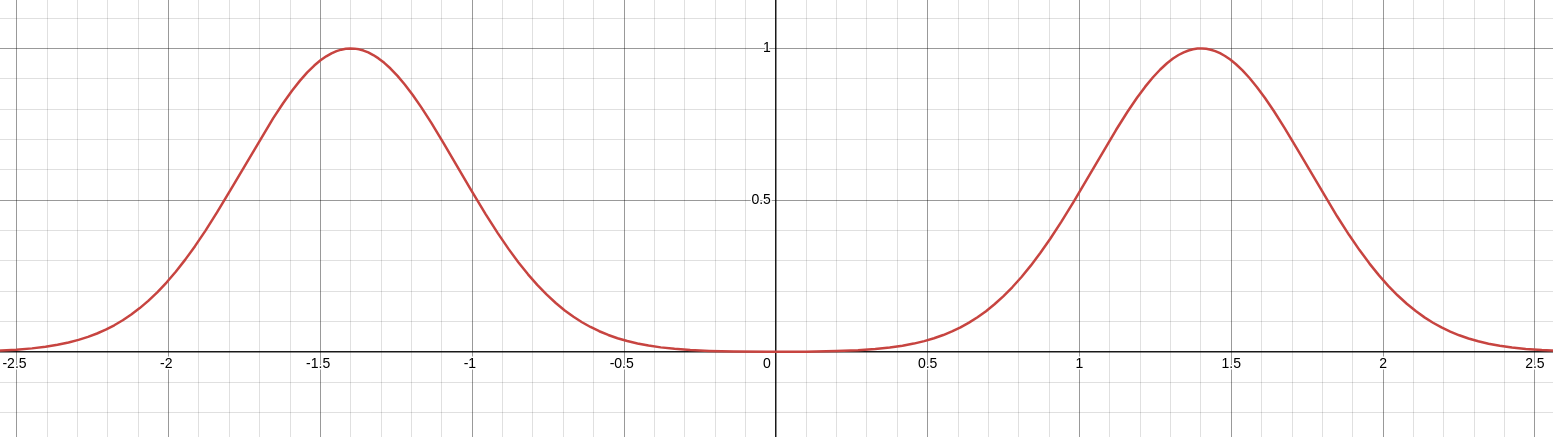
\includegraphics[width=0.9\textwidth]{fig/densi_spec_sym}
	\caption{Exemple de densité spectrale d'un signal réel ESP A 1,4}
	\label{fig:densi_spec_sym}
\end{figure}
\\
Même problème avec la covariance qui sera toujours nulle pour les signaux réels. De là en conclure que la fréquence instantanée de n'importe quel signal réel est toujours décorrélée du temps serait, pour le moins, insatisfaisant.
\\

Pour résoudre les problèmes lié à la fréquence moyenne et la largeur de bande, il suffirait de ne conserver que la partie positive du signal. On s'intéresserait alors au signal transformée $\mathcal{A}[x]$ tel que :
\[\mathcal{F}\big(\mathcal{A}[x]\big) = 2\one_{\R^+}\hat{x}\]
où $\one_E$ est la fonction indicatrice de l'ensemble $E$ et où le facteur 2 permet de conserver l'énergie du signal.
Avec la transformée de Fourier inverse, ce nouveau signal s'écrit alors :
\[\mathcal{A}[x] = \mathcal{F}^{-1}\big( 2\one_{\R^+}\hat{x} \big) = 2 \mathcal{F}^{-1}\big(\one_{\R^+}\big) * x\]
Cette indicatrice (qui n'est autre que la fonction de Heavyside) n'est pas définie au sens classique, mais l'est au sens des distributions. Pour l'écrire, on introduit la distribution suivante :
\\

\begin{definition}[valeur principale de Cauchy]\label{def:vp&Hilb}
	On appelle \emph{valeur principale de Cauchy} la distribution notée vp$\frac{1}{x}$ et définie par le crochet de dualité :
	\begin{equation}
		\forall \varphi\in\mathcal{S}(\R),\ \left\langle \text{vp}\frac{1}{x}, \varphi \right\rangle = \fint_0^t \frac{\varphi(t)}{t}dt := \lim_{\varepsilon\lr0^+} \int_{-\infty}^{-\varepsilon} \frac{\varphi(t)}{t}dt + \int_{+\varepsilon}^{+\infty} \frac{\varphi(t)}{t}dt
	\end{equation}
	Ici $\mathcal{S}(\R)$ est l’espace de Schwartz des fonctions $C^\infty$ à décroissance rapide et la limite en $\varepsilon$ assure que l'intégrale (impropre) converge bien. Sa valeur est également appelée \emph{valeur principale} de l'intégrale. 
\end{definition}

La distribution vp$\frac{1}{x}$ est appelé valeur principale dans le sens où elle conserve les propriété de la fonction inverse , dans le sens où sont produit avec l'identité donne 1 $\big(\left\langle id_\R \times \text{vp}\frac{1}{x}, \varphi \right\rangle = \left\langle \text{vp}\frac{1}{x}, id_\R \times\varphi \right\rangle=1\big)$ mais avec des propriétés d'intégration supplémentaires. Entre autre :
\\

\begin{propriete}\label{prop:fou2vp}
	La transformée de Fourier de la valeur principale de Cauchy est donnée, au sens des distributions, s'écrit avec la fonction signe :
	\begin{equation}
		\mathcal{F} \left(\text{vp} \frac{1}{x} \right)= -i \pi\, \sign{} 
	\end{equation}
	On en déduit la transformée de Fourier inverse :
	\begin{equation}
	\mathcal{F}^{-1}\big( 2\one_{\R^+} \big) = \mathcal{F}^{-1}\big( 1 + \sign \big) = \delta + \frac{i}{\pi} \text{vp}\frac{1}{x}
	\end{equation}
	
	\begin{demo}
		juste pour le plaisir. Par définition, la transformée de Fourier de la valeur principale est telle que,\\ $\forall \varphi\in\mathcal{S}(\R)$ :
		\begin{align*}
		\left\langle \mathcal{F} \left(\text{vp} \frac{1}{x} \right), \varphi \right\rangle = \left\langle \text{vp} \frac{1}{x}, \hat{\varphi} \right\rangle 
		&= \fint_\R \frac{\hat{\varphi}(\nu)}{\nu} d\nu \\
			&= \int_0^{+\infty} \frac{\hat{\varphi}(\nu) - \hat{\varphi}(-\nu)}{\nu} d\nu \\
			&= \int_0^{+\infty} \frac{1}{\nu} \left( \int_\R\varphi(t)e^{-2i\pi \nu t}dt - \int_\R\varphi(t)e^{2i\pi \nu t}dt \right)d\nu \\
			&= \int_0^{+\infty} \frac{1}{\nu}\int_\R\varphi(t)\big(e^{-2i\pi \nu t} - e^{2i\pi \nu t}\big)dt\, d\nu \\
			&= \int_0^{+\infty} \frac{1}{\nu}\int_\R-2i\varphi(t)\sin(2\pi \nu t)dt\, d\nu \\
			&= -2i\int_\R\varphi(t)\int_0^{+\infty} \frac{\sin(2\pi \nu t)}{\nu}d\nu\, dt
		\end{align*}
		En posant $u=2\pi\nu t\sign(t)$ (le signe de $t$ assure que l'on ait le même signe dans et hors du sin), on obtient :
		\begin{align*}
		\left\langle \mathcal{F} \left(\text{vp} \frac{1}{x} \right), \varphi \right\rangle &= -2i\int_\R\varphi(t)\int_0^{+\infty} \sign(t)\frac{\sin(u)}{u}du\, dt \\
		&= -2i\int_\R\varphi(t)\frac{\pi}{2}\sign(t), dt \\
		&= \big\langle -i\pi\sign, \varphi \big\rangle
		\end{align*}
	\end{demo}
\end{propriete}

\begin{definition}[transformée en SA et de Hilbet]
	On définie alors la \emph{transformée en signal analytique} (SA) du tout signal $x$ par l'application :
	\begin{equation}\label{eq:transfo_SA}
		\mathcal{A}[x] \defeq 2 x*\mathcal{F}^{-1}\big(\one_{\R^+}\big) :\ \begin{aligned} 
			\R \quad &\lr\qquad\quad \C \\	
			t\quad &\longmapsto\ x(t) + \frac{i}{\pi}\fint_\R \frac{x(s)}{t-s}ds
		\end{aligned}
	\end{equation}
	Par construction, on a bien $\mathcal{F}\big(\mathcal{A}[x]\big) = 2\one_{\R^+}\hat{x}$, est on dit plus généralement de tout signal vérifiant cette propriété que c'est un \emph{signal analytique}.
	\\
	L'intégral à droite est appelle \emph{transformée de Hilbert} du signal. Elle est notée :
	\begin{equation}\label{eq:transfo_Hilb}
		\mathcal{H}[x] :\ \begin{aligned} 
			\R \quad &\lr\qquad\quad \C \\	
			t\quad &\longmapsto\ \frac{1}{\pi}\fint_\R \frac{x(s)}{t-s}ds =  \frac{1}{\pi}\left(\text{vp}\frac{1}{x}\right)*x
		\end{aligned}
	\end{equation}
\end{definition}

Par souci de commodité, plutôt que redéfinir tout le vocabulaire développé plus haut (fréquence/temps moyen, \etc) pour les signaux réel via la transformation $\mathcal{A}$, dans la suite du mémoire on travaillera directement avec $\mathcal{A}[x]$ (et on verra que c'est essentiel).




\subsection{Propriété et interprétation des signaux analytiques}


Dans les cas des signaux réels, la transformée de Hilbert est à valeur dans $\R$. Aussi, la transformée $\mathcal{A}[x]$ à pour partie réelle $x$ et pour partie imaginaire $\mathcal{H}[x]$. Sous forme exponentielle, on a encore :
\[\mathcal{A}[x](t) = a(t)e^{i\phi(t)}\quad \Lr\quad \left\{\begin{aligned}x(t) &= a(t) \cos\phi(t) \\\mathcal{H}[x](t) &= a(t) \sin\phi(t)
\end{aligned}\right.\]
\\

\begin{definition}[Amplitude et phase]\label{def:ampli&phase_cano}
	On obtient alors on décomposition de $x$ en une paire $(a,\phi)$ telle que discuté plus haut. On définie ainsi l'\emph{amplitude} et la \emph{phase}  dite \emph{canonique} --- bien que le terme ne soit pas complètement approprié --- du signal $x$ comme étant respectivement l'amplitude et la phase de $\mathcal{A}[x]$ :
	\begin{align}\label{eq:ampli&phase_cano}
		a_x &= \big|\mathcal{A}[x]\big|   &   \phi_x &= \arg\big(\mathcal{A}[x]\big)
	\end{align}
\end{definition}



\begin{itemize}
	
	\item Il est important de noter que si un signal s'écrit sous la forme  $x=a\cos\phi$, rien n'implique $(a,\phi)=(a_x,\phi_x)$. Si ce n'est pas le cas, c'est que la première décomposition n'est ``pas la bonne''
	
	\item Exemple pour dire que les hautes fréquences partes dans la phase
	
	\item théorème de Bedrosian \cite{venouziou_characterizing_2008}
	
	\item cas AM-FM

\end{itemize}




\section{Réflexion autour du produit hermitien}


Soit $x,y\in\C^n$ des vecteurs complexes et $X,Y\in\R^{2\times n}$ leur versions réelles. On note $x^j$ sa $j^{eme}$ composante complèxe et $x_1$ (resp. $x_2$) le vecteur composé de ses parties réelles (resp. imaginaires) :
\[x = \big(x^j\big)_j =  x_1 + ix_2 =  \big(x^j_1\big)_j +i \big(x^j_2\big)_j\]
\\
On a deux façon d'écrire le produit hermitien (canonique) de $X$ avec $Y$ :
\begin{align*}
	\langle x,y \rangle = \langle x_1 + ix_2, y_1 + iy_2\rangle &= \langle x_1, y_1\rangle - i \langle x_1,y_2\rangle +i\langle x_2, y_1\rangle + \langle x_2, y_2\rangle  \\
	&= \langle x_1, y_1\rangle + \langle x_2, y_2\rangle 
	+ i\big(\langle x_2, y_1\rangle - \langle x_1,y_2\rangle\big) \\
	&= \sum_j x^j_1 y^j_1+ x^j_2 y^j_2
	+ i\left(\sum_j x^j_2 y^j_1 -  x^j_1y^j_2\right) \\
	&= \left\langle \begin{pmatrix} x_1 \\ x_2 \end{pmatrix},\begin{pmatrix} y_1 \\ y_2 \end{pmatrix}\right\rangle
	+ i\left\langle \begin{pmatrix} x_1 \\ x_2 \end{pmatrix},\begin{pmatrix} -y_2 \\ y_1 \end{pmatrix}\right\rangle \\
	&= \Big\langle X,Y\Big\rangle 
	+ i\left\langle X,\begin{pmatrix} 0 & -I_n \\ I_n & 0 \end{pmatrix}\begin{pmatrix} y_1 \\ y_2 \end{pmatrix}\right\rangle\\
	&= \Big\langle X,Y\Big\rangle 
	+ i\left\langle X,\begin{pmatrix} 0 & -I_n \\ I_n & 0 \end{pmatrix}Y\right\rangle
\end{align*}
\\
Cette formule peut s’interpréter en disant que le produit hermitien encode le produit scalaire entre $X$ et $Y$ et le produit scalaire de $X$ avec les vecteurs $y^j=(y^j_1, y^j_2)$  auquel on aurait applique une rotation de $90^\circ$ (rotation qui, par ailleurs, correspond à la multiplication par $i$ dans le plan complexe). Moralement, $\langle x,y \rangle =0$ demande une orthogonalité de $X$ à un plan, ce qui fait sens puisque cela tient compte du fait que les $x^j, y^j$ sont complexes (donc de dimension 2 en tant que $\R-$e.v.).
\\
On a aussi l'écriture (quand-même moins clair) :
\begin{align*}
	\langle x,y \rangle &= \langle x_1, y_1\rangle + \langle x_2, y_2\rangle 
	+ i\big(\langle x_2, y_1\rangle - \langle x_1,y_2\rangle\big) \\
	&= \sum_j x^j_1 y^j_1+ x^j_2 y^j_2+ i\sum_j \big( x^j_2 y^j_1 - x^j_1y^j_2 \big) \\
	&= \sum_j \big\langle X^j,Y^j\big\rangle - i\sum_j \det(X^j, Y^j)
	%&= \sum_j \|X^j\|\|Y^j\| \cos \widehat{X^j,X^j} + i\sin \widehat{X^j,Y^j}
\end{align*}
Cette formule dit que les parties reélles et imaginaires du produit $\langle x,y \rangle$ encodent respectivement ``l'orthogonalité moyenne'' et la ``linéarité moyenne ''entre les familles de vecteurs $X^j\in\R^2$ et $Y^j\in\R^2$. L'orthogonalité d'une part parce que le produit scalaire s'annule en cas d'orthogonalité (no shit), la linéarité d'autre part car le déterminant s'annule en cas de colinéarité et moyenne car se sont des sommes sur $j$. \textbf{$\bf{\langle x,y \rangle=0}$ ne dit pas que les le vecteurs sont à la fois colinéaire et orthogonaux parce que ce sont des valeurs moyennes (\ie annuler une somme ne veut pas dire que chacun des termes sont nuls).}
\\

Si maintenant on s'intéresse au cas $y=x$, on a $\forall h\in\C^n$ :
\begin{align*}
	\langle x+h, x+h \rangle = \langle x, x \rangle + \langle x, h \rangle + \langle h, x \rangle + \langle h, h \rangle 
	&= \langle x, x \rangle + \langle x, h \rangle  + \congu{\langle x, h \rangle }+ \langle h, h \rangle \\
	&= \langle x, x \rangle + 2\Re e \langle x, h \rangle + \langle h, h \rangle
\end{align*}
Donc si $x\in\C^n$ est fonction d'un paramètre $t$, l'égalité $\ \langle x, \dot{x} \rangle = \frac{1}{2}\partial_t\langle x, x \rangle\ $ du cas réel devient :
\[\langle x, \dot{x} \rangle = \frac{1}{2}\partial_t\langle x, x \rangle + i\left\langle X,\begin{pmatrix} 0 & -I_n \\ I_n & 0 \end{pmatrix}\dot{X}\right\rangle\]
\\
En particulier, quand bien-même $x$ serait de norme constante, on aurait toujours un degré de liberté pour $\ \langle x, \dot{x} \rangle$ :
\[\|x\|=c\quad \Lr\quad \langle x, \dot{x} \rangle = i\left\langle X,\begin{pmatrix} 0 & -I_n \\ I_n & 0 \end{pmatrix}\dot{X}\right\rangle\]
\\

\begin{definition}\label{def:phase_dyn}
	Ainsi, il reste tout un degré de liberté au produit $\ \langle x, \dot{x} \rangle\ $ même si $x\in\S^{2n}$. En intégrant ce degré de liberté supplémentaire, c'est-à-dire en tenant compte de son évolution sur la période $[t_0,t]$, l'on obtient ce qui est appeller le \emph{phase dynamique} :
	\[\phased \defeq \phased(t_0,t) = \int_{t_0}^t \Im m \big\langle \psi(s) \, |\, \dot{\psi}(s) \big\rangle ds\]
	Elle dynamique en cela qu'elle est propre au variation de $\psi$ et qu'elle considère tout l'évolution de $\psi$ : ça dynamique.
	\textit{Rq} : Avec les notations de la \cref{sec:temp-freq} et si le signal est d'amplitude constante, alors on a :
	 \[\phased(-\infty, +\infty) = \int_\R \big\langle \psi(s) \, |\, \dot{\psi}(s) \big\rangle ds = -2\pi\int_\R \nu\big|\hat{\psi}(\nu)\big|^2 d\nu = - 2\pi \esp[|\hat{\psi}|^2]{\nu}\]
	
	\textbf{... et pourquoi c'est une PHASE du coup ?}
\end{definition}


\begin{definition}[Connexion de Berry]\label{def:berry_connx}
	On appelle \emph{connexion de Berry} le champ de forme linéaire :
	\begin{equation}\label{eq:berry_connx}
		\forall \psi\in\mathpzc{M},\quad A_\psi :\ \begin{aligned} T_\psi\mathpzc{M}\ &\lr\qquad\ \R \\ \phi\quad &\longmapsto\ \Im m \big\langle \psi(s) \, |\, \phi(s) \big\rangle
		\end{aligned}
	\end{equation}
	\textbf{Elle a rien d'une connexion par contre :/}
\end{definition}





\setcounter{section}{0}
\setcounter{figure}{0}
\setcounter{lstlisting}{0}

\part{Phase Géométrique}

\section{Description des signaux multivariés}\label{sec:bases}




\subsection{Version Lilly \cite{lilly_bivariate_2010, lilly_analysis_2012}}

\begin{itemize}
	\item On veut écrire $\bf{x}$ sous la forme :
	\[\bf{x}(t) = a(t)e^{i\phi(t)}\begin{pmatrix} a_1(t)e^{i\phi_1(t)} \\ a_2(t)e^{i\phi_2(t)} \\ \vdots \\ a_n(t)e^{i\phi_n(t)}
	\end{pmatrix}\]
	
	\item Lilly explique comment obtenir $\phi$ dans le cas général (faut revoir ça parce que meh quand-même)
	
	\item Sauf que ce $\phi$ c'est lié à la phase dynamique est pas du tout à polarisation du signal. Pourtant c'est dans la polar qu'on a la phase géo.
	
	\item Quoi qu'il en soit, les cas dim 2 et 3 c'est fait \cite{lilly_wavelet_2006, lilly_bivariate_2010, lefevre_polarization_nodate}
\end{itemize}

\subsection{Cas bivarié et trivarié}
On a un signal bivarié $\bf{x}(t) = \big(x(t),y(t)\big)$ qu'on transforme (voir \cref{subsec:SA_Hilb}) soit la forme :
\[z_x(t) = \begin{pmatrix}x_+(t) \\ y_+(t)\end{pmatrix} = \begin{pmatrix}a_x(t) e^{i\phi_x(t)} \\ a_y(t) e^{i\phi_y(t)}\end{pmatrix}\in\C^2\]
\\

\`A côté de ça, on a les ellipses modulées :
\[z(t) = e^{i\theta}\big(a(t)\cos\phi(t) + ib(t) \sin\phi(t)\big) = A(t) e^{i\theta} \big( \sin\chi(t) \cos\phi(t) + i\sin\chi(t) \sin\phi(t) \big) \in\C\]
Qui sous forme vectoriel se réécrit :
\begin{equation}\label{eq:exp_elliptik}
	z(t) = e^{i\phi} R_{\theta(t)}\begin{pmatrix} a(t) \\ -ib(t) \end{pmatrix} = A(t)e^{i\phi} R_{\theta(t)} \begin{pmatrix} \cos\chi(t) \\ -i\sin\chi(t) \end{pmatrix} \in\C^2,\qquad R_\theta\in\SO_2(\R) \
\end{equation}
\\

Pour avoir la désinscription de $\bf{x}$ en terme d’ellipse, il suffit donc de poser :\footnote{C'est la version analytique du la version vectorielle de l'ellipse !}
\[z_x(t) = z(t)\quad \Llr\quad \begin{pmatrix}a_x(t) e^{i\phi_x(t)} \\ a_y(t) e^ {i\phi_y(t)}\end{pmatrix} = A(t)e^{i\phi} R_{\theta(t)} \begin{pmatrix} \cos\chi(t) \\ -i\sin\chi(t) \end{pmatrix}\]
\\
Ensuite, on pose :
\[\begin{pmatrix}z_+ \\ z_-\end{pmatrix} = \begin{pmatrix}a_+ e^{i\phi_+} \\ a_- e^{i\phi_-}\end{pmatrix} = \frac{1}{2}\begin{pmatrix}x_+ + iy_+ \\ x_+ - iy_+\end{pmatrix} = \frac{1}{2}\begin{pmatrix}1 & i \\ 1 & -i\end{pmatrix} \begin{pmatrix}x_+ \\ y_+\end{pmatrix}\]
\\
Et on a :
\begin{align*}
	2\phi &= \phi_+ + \phi_-  &  a &= A\cos\chi = a_+ + a_- \\
	2\theta &= \phi_+ - \phi_-  &  b &= A\sin\chi = a_+ - a_- 
\end{align*}
et on en déduit :
\begin{align*}
	A &= \sqrt{(a_+ + a_-)^2 + (a_+ - a_-)^2}  &  \begin{aligned} \cos\chi &= \frac{a_+ + a_- }{\sqrt{(a_+ + a_-)^2 + (a_+ - a_-)^2}}  \\  \sin\chi &= \frac{a_+ - a_- }{\sqrt{(a_+ + a_-)^2 + (a_+ - a_-)^2}}	\end{aligned}
\end{align*}
Ce qui donne \infine :
\[\begin{pmatrix}x_+ \\ y_+\end{pmatrix} = e^{i\frac{\phi_+ + \phi_-}{2}} R_{\frac{\phi_+ - \phi_-}{2}} \begin{pmatrix}a_+ + a_- \\ -i(a_+ - a_-)\end{pmatrix}\]
\\

L'\cref{eq:exp_elliptik} ce généralise  très bien, il suffit d'augmenter la taille de $R_\theta\in\SO_n(\R)$ et de lui donner le vecteur étendu :\footnote{\textit{Sachant que le vecteur contenant $a$ et $b$ est principalement nul, on peut réécrire le produit ne considérant que les deux premières colonnes de $R_\theta$.}}
\[z_x(t) = \begin{pmatrix}x_{1+}(t) \\ \vdots \\ 
	x_{n+}(t)\end{pmatrix} = e^{i\phi} R_{\theta(t)}\begin{pmatrix} a(t) \\ -ib(t) \\ 0 \\ \vdots \\ 0 \end{pmatrix} = A(t)e^{i\phi} R_{\theta(t)} \begin{pmatrix} \cos\chi(t) \\ -i\sin\chi(t) \\ 0 \\ \vdots \\ 0 \end{pmatrix}\]
\\

Maintenant, la question est de savoir comment généraliser la transformation en $(z_+, z_-)$ pour obtenir les paramètres $(A, \phi, R_\theta, \chi)$ dans ce cas...
\\
Pour généraliser le procédé, on peut noter que :
\[\begin{pmatrix}z_+ \\ z_-\end{pmatrix} = \frac{1}{2}\begin{pmatrix}1 & i \\ 1 & -i\end{pmatrix} \begin{pmatrix}x_+ \\ y_+\end{pmatrix} = \frac{1}{\sqrt{2}}U \begin{pmatrix}x_+ \\ y_+\end{pmatrix}\qquad\qquad \text{avec }\ U=\frac{1}{\sqrt{2}}\begin{pmatrix}1 & i \\ 1 & -i\end{pmatrix}\in\U(2)\]
\\ 
Ce qui ramène à se demander comment généraliser $U$ à $\SU(n)$. Le problème est que $U$ est indépendant de tout les paramètres $(A, \phi, R_\theta, \chi)$ et sa généralisation est vraiment pas évidente sachant qu'on que le formule avec $n=2$... et pour $n=3$ ca devient déjà chaud (pour rappelle $\dim \SO_n(\R)=\frac{n(n-1)}{2}$ et donc $\theta\in\R^n$, ce qui rend le problème de pire en pire à mesure qu'on augmente $n$).



\subsection{Mon blabla}\label{subsec:blabla}


\begin{definition}[Signal multivarié] \label{def:signal_multivar}
Un \emph{signal multivarié}, ou \emph{$n-$varié}, est un signal à valeur dans $\C^n$. Formellement, c'est une fonction de carré intégrable (or is it ?) à valeur de $\R$ dans $\C^n$, et l'ensemble de tel signaux seront noté $L^2\big(\R,\C^n\big)$.
\\
Dans le cas $n=2$, on parle de signal \emph{bivarié}.
\end{definition}

\begin{enonce}[PVD Optimisation]
	Lilly \cite[p. 602/3]{lilly_analysis_2012} obtient la phase instentanée en minimisant l'erreur d'approximation :
	\[v^2(t,\omega(t)) = \frac{\|\Tilde{x}(t,\omega(t))\|^2}{\|x(t,\omega(t))\|^2}\]
	Ce qui lui donne :
	\[\omega(t) = \phi(t)/\tau = \Im m\langle \overline{x}, x'\rangle\]
	
	QUESTION : est-ce qu'on peut tout avoir en minimisant la bonne quantité ? (oui, principe de moindre action frr)
\end{enonce}

\begin{proposition}\label{prop:quatern}
Les signaux bivariés se décrivent très simplement à l'aide des quaternions. En considérant $\{1, \bf{i},\bf{j},\bf{k}\}$ la base canonique des quaternions $\mathbb{H}$, on peut voir $\psi$ comme étant à valeur dans ${\C_{\bf{j}}}^n$ ($\C_{\bf{j}} :=\R\times \bf{j}\R$), de sorte que :
\[\forall \psi\in L^2(\R,\mathbb{H}),\ \exists a,\theta,\chi,\varphi \in\mathcal{C}(\R)\ |\quad \psi(t) = a(t)e^{\bf{i}\theta(t)}e^{-\bf{k}\chi(t)}e^{\bf{j}\varphi(t)}\]
\\
Sous cette forme, les paramètres $a$ et $\varphi$ s'interprètent respectivement comme l'amplitude et la phase instantanée du signal. Les deux paramètres restant contrôle l'ellipticité ($\chi$) et l'orientation ($\theta$) de l’ellipse de polarisation instantanée. C'est-à-dire l'ellipse que suit la signal à l'instant $t$.
\\
Dit autrement, à tout instant $t$, $\psi(t)$ est vu comme une point d'une ellipse dont la taille est caractériser par $a(t)$, l'ellipticité par $\chi(t)$ et l'orientation par $\theta(t)$. $\phi(t)$ permet lui de situer $\varphi(t)$ sur cette ellipse.
\\

\textit{Le problème de cette représentation est qu'elle se généralise mal aux signaux plus que $2-$variés et, à notre connaissant, il n'existe pas d'extensions des quaternions à de plus haute dimension. voir \cref{prop:gene_param_signal_v1,prop:gene_param_signal_v2}, \cref{eq:phase_tot,,eq:phase_dyn,eq:phase_geo}} 
\end{proposition}

Il est évident que cette représentation est présent bien plus de paramètre que nécessaire, puisse que deux devrait suffire. Pour autant, elle permet de mieux \textbf{je sais quoi mais c'est sur qu'il y'a une raison}.
\\
Si cette représentation se généralise mal parce qu'elle demanderait d'avoir une extension de $\mathbb{H}$, sont interprétations graphique, elle, se généralise très bien. Par exemple, en dimension 3, alors l'ellipse devient une ellipsoïde. L'amplitude reste de dimension 1 parce qu'elle ne fait que contrôler la taille de cet ellipsoïde, mais les autres paramètres eux doivent être de dimension 2. L'ellipsoïde à besoin de deux angles pour être orienté, possède deux degrés d'ellipticité et ces points sont déteminés par deux angles.
\\

\begin{proposition}\label{prop:gene_param_signal_v1}
Plus généralement, tout signal multivarié $\psi$ est (\textit{devrait être}) caractérisé par quatre paramètres (donc $1+(n-1)(\frac{n}{2}-2)$ scalaires) :
\begin{align*}
	a&\in\mathcal{C}(\R,\R^+)  &  \theta&\in\mathcal{C}(\R, [-\pi/2,\pi/2]^{\frac{n(n-1)}{2}})  &  \chi&\in\mathcal{C}(\R, [-\pi/4,\pi/4]^{n-1})  &  \varphi&\in\mathcal{C}(\R, [-\pi,\pi]^{n-1})
\end{align*}	
\end{proposition}

\`A bien y réfléchir, décrire un ellipsoïde dans l'espace, c'est exactement de que font les matrices symétriques définies positives. Donc on pourrait tout à fait remplacer les informations $(a,\theta,\chi)$ par une matrice symétrique positive de dimension $n$. Il ne resterait alors plus que $\varphi$ qui, de toute façon ne devrait pas trop être lié aux autres paramètres.

Enfin, surement que si parce que y'a un monde pour $\varphi=0_\R^n$ et c'est le reste des paramètres qui fait le travail. Mais clairement c'est pas intéressant comme description. L'idée serait plutôt décrire le signal $\psi$ en minimisant les variations de $(a,\theta,\chi)$.
Ca appelle clairement à chercher que dans l'espace de Siegel mais pas seulement, parce que c'est pas juste des chemins chez Siegel qui nous intéresse.

Ou alors c'est le jeu de jauge qui fait qu'on tue $\varphi$ ? auquel cas tout les jours Siegel.
\\

\textit{BTW, les quaternions c'est fait pour décrire les rotations et c'est (quasiment) ce qu'on fait avec, donc aller chercher dans un espace de matrices pour généraliser le principe c'est pas déconnant.}
\\
\textit{D'ailleurs, vu que c'est pas exactement ce qu'on fait avec, dans quelle mesure c'est pas le cas et est-ce qu'on exploite vraiment la structure des quaternions ?}
\\ 

\begin{proposition}\label{prop:gene_param_signal_v2}
Autre approche : un signal multivarié étant moralement un chemin de $\R^n$, son graphe est une variété (plongée) de dimenion 1. Sachant cela, si en chaque instant on veut définir l'ellipsoïde sur laquelle elle repose à un insant $t$, il est morale que cette ellipsoïde soit en fait une ellipse puisque c'est elle-même une variété de dimension 1.
\\
Partant de là, on aurait toujours $a$, $\chi$ et $\phi$ pour la décrire et seulement $\theta$ gagnerait en dimension pour pouvoir orienter l'ellipse dans les $n$ axes. $\psi$ serait alors la données de $3+\frac{n(n-1)}{2}$ paramètres :
\begin{align*}
	a&\in\mathcal{C}(\R,\R^+)  &  \theta&\in\mathcal{C}(\R, [-\pi,\pi]^{\frac{n(n-1)}{2}})  &  \chi&\in\mathcal{C}(\R, [-\pi/4,\pi/4])  &  \varphi&\in\mathcal{C}(\R, [-\pi,\pi])
\end{align*}
\end{proposition}

On aurait beaucoup moins de paramètre et c'est quand-même bien. En même temps ca parait plus contraignant comme modèle. Pour comparer les deux, il faudrait voir comment les deux se décomposant dans le cas d'un signal qui ne varierait sur une ellipsoïde fixe. \ie dans un cas où $\theta,\chi$ de la \cref{prop:gene_param_signal_v1} varie pas alors que ceux de la \cref{prop:gene_param_signal_v2} si.




\setcounter{figure}{0}
\setcounter{lstlisting}{0}

\section{Phase géométrique d'un signal}\label{sec:phasegeo}

La phase géométrique est invariante par action du groupe $\mathbb{U}(1)$, c'est à dire invariante par changement de la phase instantanée. Elle ne regarde donc que les paramètres $a, \theta$ et $\chi$. En outre, elle ne regarde que la matrice semi-définie positive (potentiellement sans même regarder l'amplitude $a$ a.k.a. la norme de la matrice).

Avec cette formulation il devient plus clair que $\phi$ peut être vu comme un fibré vectoriel (particulier parce que c'est bien un élément du produit $\R\times\C^n$ pas d'un espace qui s'en rapproche localement) et cette et que le groupe $\mathbb{U}(1)$ agit comme un jauge. En plus, Wikipédia dit que pour les fibrés vectoriels, il faut que l'action soit les changement de base (orthonormée ?), ce qui correspond bien à une changement de phase suivant les formules de la \cref{prop:gene_param_signal_v1}.

La question reste encore de savoir comment on détermine les $(a,\theta,\chi,\varphi)$ parce que encore une fois, y'a vraiment pas unicité de la décomposition et c'est loin d'être clair comment choisir la plus pertinente (et comment la calculer aussi !)



\section{Trucs à voir}

\subsection{Bilan des formules}

\begin{itemize}
	\item Les phases de $\psi$ entre les instants $t_0$ et $t$ :
	\begin{equation}\label{eq:phase_tot}
		\phaset(\psi, t_0, t) \equiv \arg(\psi(t_0), \psi(t))
	\end{equation}
	
	\begin{equation}\label{eq:phase_dyn}
		\phased(\psi,t_0,t) \equiv \Im m \int_{t_0}^t\big\langle \psi(s) \,|\, \dot{\psi}(s) \big\rangle ds
	\end{equation}
	
	\begin{equation}\label{eq:phase_geo}
		\phaseg(\psi, t_0, t) \equiv  \phaset(\psi, t_0, t) - \phased(\psi,t_0,t)
	\end{equation}
	
	\item (conservative) Équation Schrödinger et de Liouville-von Neumann ($h(R)$ : Hamiltonien des paramètres $R$, $W$ : opérateurs statistique ) \cite[p.6]{bohm_geometric_2003} :
	\begin{equation}\label{eq:schrodinger}
		i\frac{d \psi(t)}{dt} = h(R)\psi(t)
	\end{equation}
	\begin{equation}\label{eq:liouville-neumann}
		i\frac{d W(t)}{dt} = \big[h(R),W(t)\big] \qquad\qquad [\cdot\,,\cdot]=\text{ commutateur ?}
	\end{equation}
	
	\item Moment angulaire (viteuf) $\forall z\in\C$ :
	\begin{equation}\label{eq:mom_angu}
		M(t) = \Re e \big(iz\congu{z}'\big) = -\Im m z\congu{z}'  \qquad\qquad \text{thoughts ?}
	\end{equation}
	
\end{itemize}


\subsection{Général}

\begin{itemize}
	\item D'où sort l'interprétation géométrique + son lien avec quaternions (prop. \ref{prop:quatern})
	\item Lien avec l'eq de Schrödinger (l'intérêt de $H$ et $K$ + d'où ils sortent)
	\item J'ai rien compris au ``problème'' des formalisations vecteur et/vs complexe
	\item Comment comprendre $\big\langle \psi\, |\, \dot{\psi} \big\rangle$ ?
	
	\item La ``Berry connection'' c'est une vraie connexion ? elle est où la covariance alors ?
\end{itemize}

\[\underline{\overline{\qquad\qquad\qquad\qquad\qquad\qquad\qquad\qquad\qquad\qquad\qquad\qquad\qquad\qquad\qquad\qquad\qquad\qquad}}\]{\color{white}relbinrei}

\begin{itemize}
	\item ``horizontal lift'' : pourquoi horizontal ? en quel sens ?
	\item Fréquence de Rubi
	\item Matrice/base de Pauli et généralisation, groupe $SU(n)$ (un peu de quantique ?)
	\item Produit hermitien : intuition géométrique
	\item Monopole de Dirac + lien avec la phase géo (un peu d'électro-magnétisme ?)
	\item Invariant de Bargmann + série de Dyson
\end{itemize}



\subsection{Point de vue des variétés}\label{subsec:phaseG_variete}

\begin{itemize}
	\item Ecriture en terme de fibré (principale ? vectoriel ?)
	
	\item Choix de l'action de groupe pour la jauge : $U(1)$ \apriori
\end{itemize}

\[\underline{\overline{\qquad\qquad\qquad\qquad\qquad\qquad\qquad\qquad\qquad\qquad\qquad\qquad\qquad\qquad\qquad\qquad\qquad\qquad}}\]{\color{white}relbinrei}

\begin{itemize}
	\item Lien avec Siegel : assez clair avec la visualisation des ellipses, beaucoup moins avec les Hilberts même si $| \psi\rangle \langle \psi |\in$ Siegel \apriori
	
	\item ``\textit{Symplectique}'' (meaning + intérêt ?)
	
	\item 
\end{itemize}




\newpage

\listoffigures
\vfill
\lstlistoflistings
\vfill
%\listtheorems

\newpage

\bibliography{ref.bib}{}
\bibliographystyle{siam}
\end{document}